\documentclass[../cap1_latex.tex]{subfiles}
%Metodologia:
	


	El invernadero propuesto consta de 3 componentes; el invernadero como estructura física, el modelo de optimización el cual define el comportamiento futuro del invernadero y un sistema de gestión que realice la función de puente entre múltiples aplicaciones, el modelo y el invernadero. La interacción entre los componentes se ejemplifica en la figura \ref{fig:sistemas}.

		\begin{figure}[!ht]
			\centering
				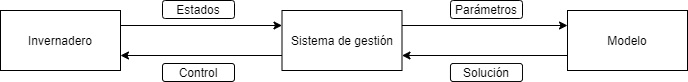
\includegraphics[width=\linewidth]{../imagenes/Sistemas.png} 
			\caption{Relación entre sistemas desarrollados}
			\label{fig:sistemas}
		\end{figure}

	\subsection{INVERNADERO}
		El invernadero desarrollado se compone tanto de la estructura física que alberga y aísla las plantas, actuadores (bombas, calefactor y luminaria) , elementos de medición (sensores) y una caja con la electrónica necesaria para la interacción de los elementos anteriores.
		
		
		\subsubsection{ESTRUCTURA}
			La estructura del invernadero se construyó en dos partes: 
			\begin{itemize}
			
			
			
				\item Una base cuadrada que sujeta y asila térmicamente a 8 contenedores (submódulos) que funcionan como macetas para las plantas mas un contenedor, estos contenedores a su vez rodean un mayor contenedor (unidad central) el cual almacena el agua, esta agua se utiliza como intercambiador de calor al moverse atravesó de las cañerías de calefacción que atraviesan de forma similar por cada uno de los 8 submódulos con retorno a la misma unidad central Figura XX , esta gua también será utilizada para la irrigación mediante SDI en cada uno de los submódulos.
				
				\item 
				Una tapa para la base con paredes transparentes y aislantes construidas como un “sándwich” de polietileno y aire, esta tapa también sujetara un cuadro suspendido de altura regulable con “tiras led” para lograr una iluminación asistida cuando la iluminación natural escasee.
			\end{itemize}
			

			\begin{figure}[!ht]%
			\centering
			\subfloat[\centering Modelo 3D]{{ 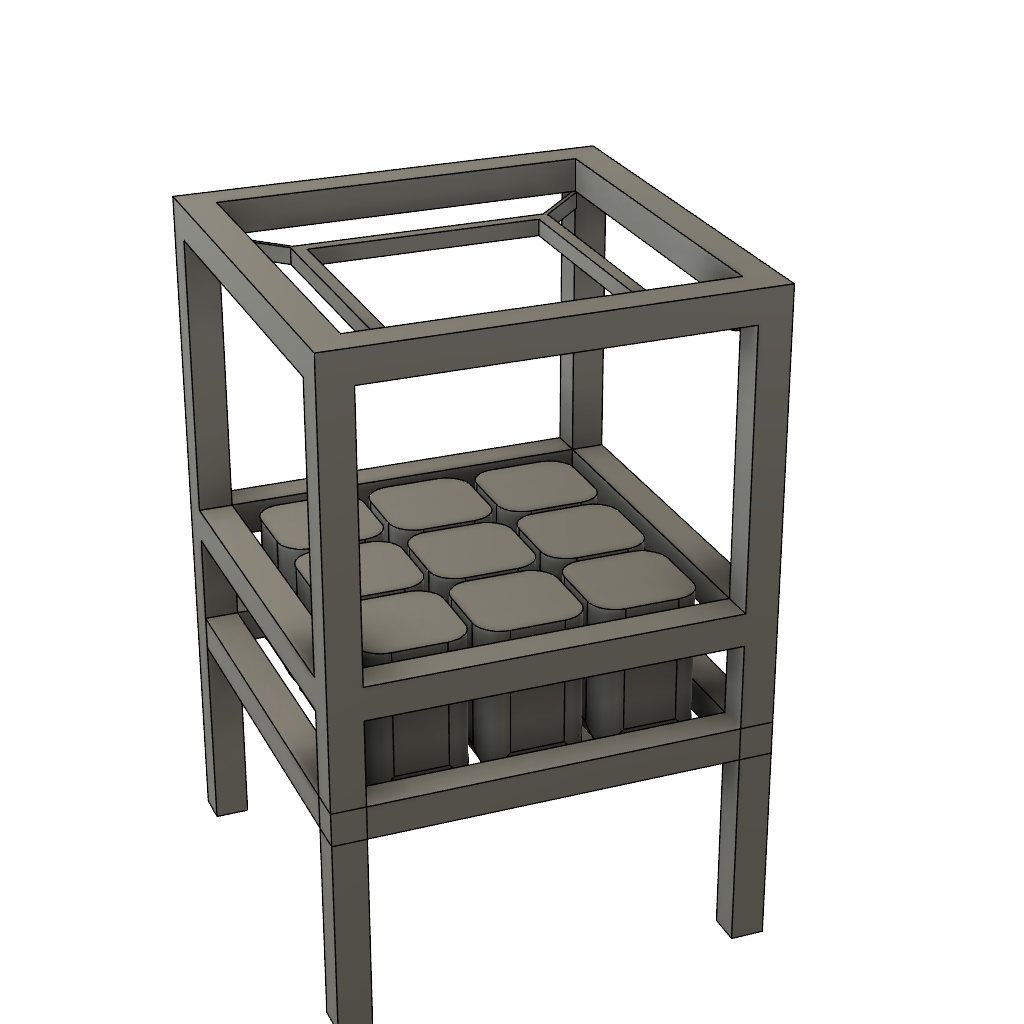
\includegraphics[width=0.45\linewidth]{../imagenes/cajon3d.png} }}%
			\qquad
			\subfloat[\centering Maqueta desarrollada]{{ \includegraphics[width=0.45\linewidth]{../imagenes/cajon.jpg} }}%		
			\caption{Modelo 3D propuesto y maqueta realizada}%
			\label{fig:maqueta}%

			\end{figure}%			

		\subsection{CAJA}
		
			al exterior de la estructura estará presente una caja estanca Figura XX que contenga los mecanismos de control para los actuadores (bombas, iluminación LED y calefactor) ubicados en el invernadero además de un microcontrolador ESP-32-WROOM el cual se encargara del manejo de señales dentro y hacia afuera del invernadero, finalmente existirá una fuente de poder que entregue los voltajes [ 3,3V : 5V : 12V ] los cuales son necesarios para los elementos de control y en paralelo a esta fuente se desviara una vía de 220V que pase atreves de los relees respectivos para el control de los actuadores de mayor potencia (calefactor y bomba) .

			\begin{figure}[!ht]
				\centering
				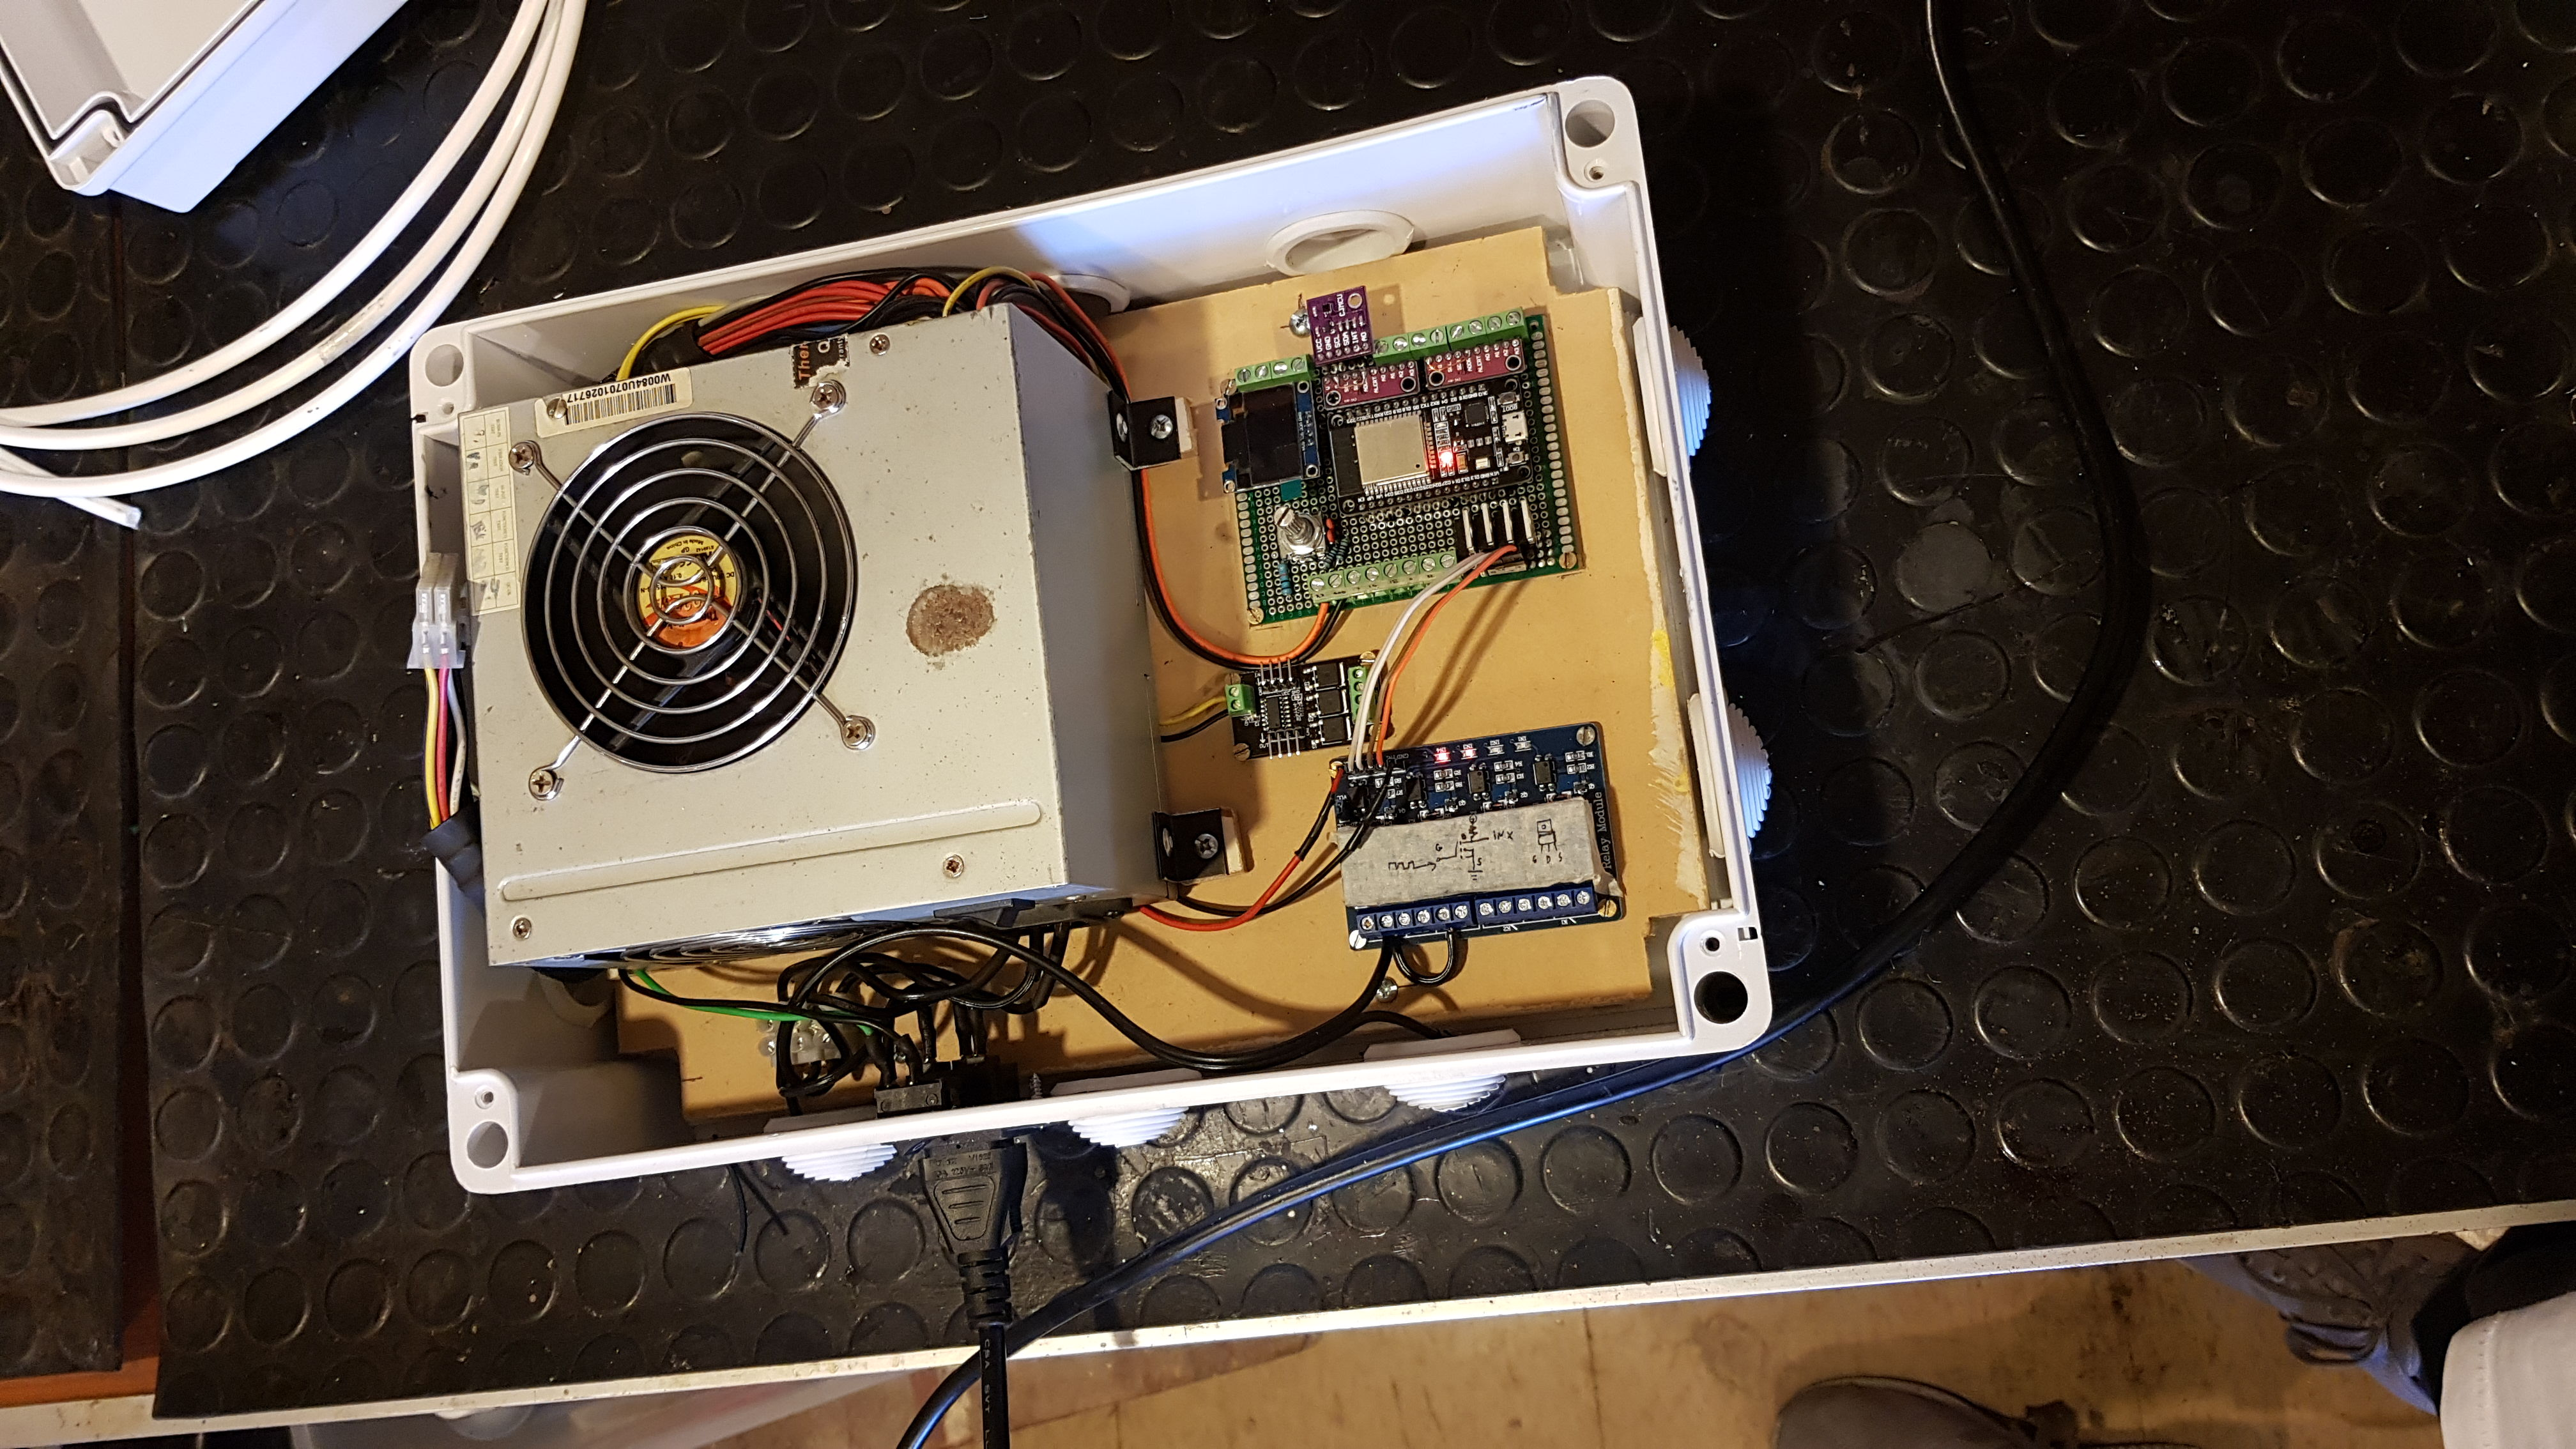
\includegraphics[width=0.75\linewidth]{../imagenes/caja.jpeg} 
				\caption{Caja con los elementos de control}
				\label{fig:flujo_agua}
			\end{figure}



		El funcionamiento del invernadero se realizará mediante el control de tres variables en su interior iluminación, temperatura e irrigación, a continuación, se describirá cada sistema y metodología de control.
		\begin{itemize}
		
		
			\item La \textbf{iluminación asistida} será controlada de forma proporcional según la iluminación resultante de la luminaria LED más la iluminación natural esperada para un tiempo determinado en el día. Para esto se utilizará el sensor de intensidad lumínica MAX44900 el cual permite una medida integrada en un tiempo de 50 ms como lo recomienda el fabricante para las condiciones en que será expuesto el sensor, además se utilizará un controlador de corriente constante P9813 para luces LED, su salida será ajustada entre cada lectura del sensor.
			\item La \textbf{irrigación} será controlada por la variable de irrigación ($BA$) que entrega el modelo, según esta se accionará la bomba de irrigación, esta acción rellenará la columna de agua que genera una presión de valor conocida sobre el tubo de goteo en el subsuelo, finalmente esta presión provocará un goteo que humedecerá la tierra de cada contenedor de forma similar, esta humedad será medida por un sensor capacitivo de humedad de salida analógica.
			El flujo de agua dentro del invernadero se puede apreciar en la Figura \ref{fig:flujo_agua}
			
			\begin{figure}[!ht]
				\centering
				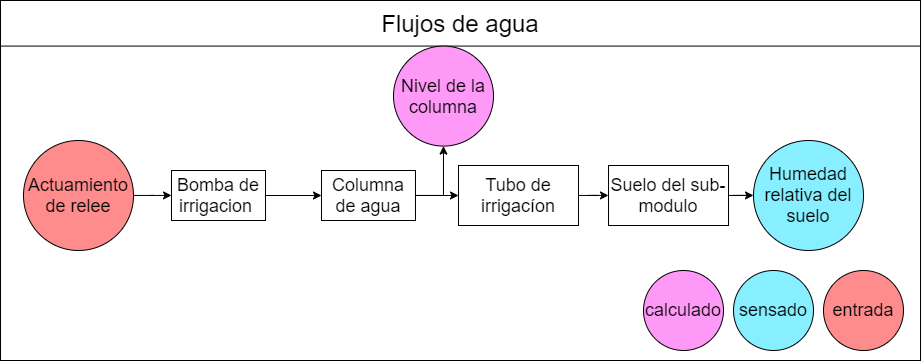
\includegraphics[width=\linewidth]{../imagenes/flujos de agua.png} 
				\caption{Relación entre sistemas desarrollados}
				\label{fig:flujo_agua}
			\end{figure}						
			
			\item La \textbf{temperatura} será regulada, al igual que la irrigación por medio del modelo matemático, donde se accionará tanto la bomba de temperatura como el calefactor según la variable de calefaccionar ($BT$), el calefactor calentara el agua del módulo principal y la bomba circulará esta agua calentada por una tubería de cobre que atraviese a cada submódulo como se presenta en la \tarea{Figura XX}, el calor se transferirá como se muestra en la Figura \ref{fig:flujo_calor}.
			
			\begin{figure}[!ht]
				\centering
				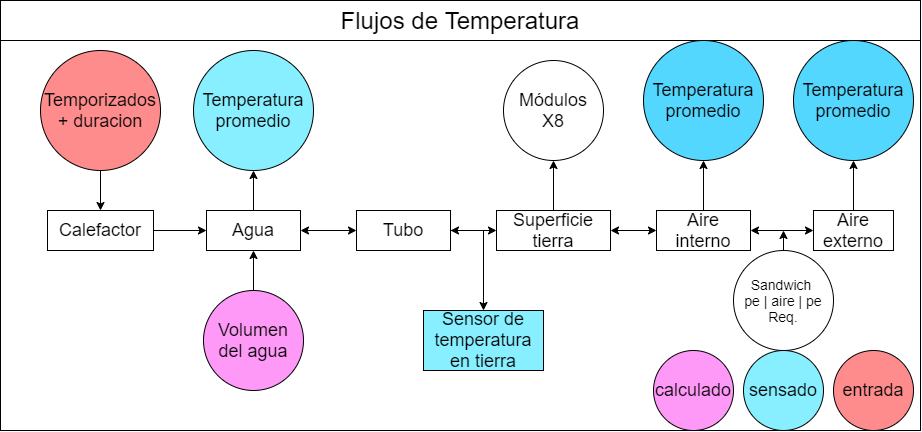
\includegraphics[width=\linewidth]{../imagenes/flujos de calor.png} 
				\caption{Relación entre sistemas desarrollados}
				\label{fig:flujo_calor}
			\end{figure}

		\end{itemize}



		
		\subsubsection{Instrumentación}	
			
			
			La instrumentación para el invernadero se encuentra descrita en el Cuadro \ref{tab:instrumentacion}.

\begin{table}[!ht]
\centering
\resizebox{\linewidth}{!}{%
\begin{tabular}{|l|l|l|l|}
\hline
Nombre            & Tipo             & Descripción                                  & Rango                                                                                                                                                                                                                                \\ \hline
DHT11             & Sensor           & Sensor de temperatura y humedad de relativa  & \begin{tabular}[c]{@{}l@{}}$ [20 \, \enleadertwodots \, 90] $ Hum relativa\\ $ [0 \, \enleadertwodots \, 50] $ C°\end{tabular} \\ \hline
MAX44009          & Sensor           & Sensor de intensidad lumínica                & $ [ 0.045   \, \enleadertwodots \,  188000  ] $ Lux                                                                                                                               \\ \hline
LM35              & Sensor           & Sensor de temperatura                        & $ [-55 \, \enleadertwodots \, 150 ] $ C°                                                                                                                                           \\ \hline
Sensor Capacitivo & Sensor           & Sensor capacitivo de humedad en el suelo     & $ [¿? \, \enleadertwodots \,  ¿? ] $ Hum relativa                                                                                                                                 \\ \hline
ADS1115           & ADC              & Conversor análogo $\rightarrow$ digital      & $ [ 16 ] $ Bits                                                                                                                                                                                                                \\ \hline
P9813             & Controlador led  & Controlador con memoria para tiras led       & $ [ 8 ] $ Bits/canal                                                                                                                                                                                                           \\ \hline
Modulo Relay's    & Relay            & Modulo relay's con señal aislada             & \begin{tabular}[c]{@{}l@{}}$ [ 4 ] $ Salidas\\ $ [ 0 \, \enleadertwodots \,  250 ] $ VAC\end{tabular}                                                                        \\ \hline
ESP32-WROOM       & Microcontrolador & Microcontrolador con conexión WIFI integrada & $ [ 3.3 ] $ Volts                                                                                                                                                                                                              \\ \hline
Calefactor        & Actuador         & Calefactor para agua en contenedores         & $ [ 75 ] $ Watts                                                                                                                                                                                                                \\ \hline
Bomba pequeña     & Actuador         & Bomba hidráulica                             & $ [ 5 ] $ Volts                                                                                                                                                                                                                 \\ \hline
Bomba grande      & Actuador         & Bomba hidráulica                             & $ [ 220 ] $ VAC                                                                                                                                                                                                                \\ \hline
\end{tabular}%
}
\caption{Componentes utilizados\label{tab:instrumentacion}}
\end{table}


	Dentro de los sensores utilizados, se destaca que tanto los MAX44009 como los ADS1115 fueron conectados por medio del protocolo I2C lo que permitió un mejor aprovechamiento de los pines del ESP32. También se debe destacar, que al utilizarse la funcionalidad de conexión WIFI en el microcontrolador, este deja de tomar medidas exactas por su ADC interno y por ello se utilizó el ADS1115.Otro caso importante de mencionar es el del DHT11 el cual es un sensor con un tiempo de muestreo lento (2 segundos entre mediciones), el cual debe respetarse ya que este puede enviar información antigua sin alerta alguna o incluso puede perder la siguiente medición si se le apura mucho. 
	

	
	
	

	\subsection{Sistema de gestión}
	
	

	
	
		Para la realización de la automatización de este proyecto se utilizó el protocolo sobre TCP MQTT, el cual permite la comunicación entre muchos dispositivos. Una base de datos MySQL que almacenaría la información relevante respecto al o los invernaderos, además de otras herramientas desarrolladas para la gestión del invernadero de forma sencilla. También, se realizó un sistema de control cerrado en el caso de que el invernadero no reciba información del servidor y por ende el control determinado por el modelo matemático.
		
		
		
			
	
		\subsubsection{Mosquitto(MQTT) \& MySQL}
			Las herramientas ya existentes que se utilizaron fueron:
				\begin{itemize}
					\item Boker de MQTT Mosquitto, el cual es una herramienta gratuita con varias opciones de seguridad y configuración para el caso de este proyecto. Todas las comunicaciones se realizarán por websocket con autentificación de usuarios para mantener un control sobre aquellos dispositivos que envían y/o reciben mensajes de cada tópico.
					\item Base de datos MySQL, en la cual se configuró un usuario con acceso restringido tanto para editar como visualizar las tablas que contendrán la información respecto al invernadero, además de otro usuario quien solo podrá visualizar dichas tablas, con el objetivo de tener protegida la base de datos, ya que solo se tendrá una instancia local que aceda a la edición de las tablas y muchos posibles clientes que visualicen la información de forma no local.
				\end{itemize}							

			
	
	
		\subsubsection{Parser MQTT $ \rightarrow $ SQL}
			\label{parser}
			Debido a los múltiples tipos de mensajes que pueden ser transmitidos dentro de los tópicos del MQTT se optó por seguir un protocolo conocido para él envió de mensaje "JSON"  (Javascript object notation), de esta forma es más simple ordenar el contenido de los mensajes, además de entregar información relevante respecto a este. Los mensajes se encuentran descritos en la Figura \ref{fig:mensajes}.
			
			\begin{figure}[!ht]
				\centering
				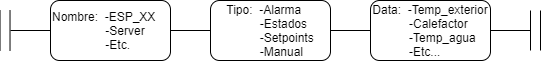
\includegraphics[width=\linewidth]{../imagenes/mensajes.png} 
				\caption{Formato de los mensajes dentro del MQTT}
				\label{fig:mensajes}
			\end{figure}
			
			Ya que los mensajes solo estarán disponibles dentro de los tópicos del MQTT, se realizó una aplicación en Java que realice lo siguiente:
			\begin{itemize}
				\item Conectarse a los tópicos relevantes (entradas y salidas).
				\item Procesar el mensaje en JSON a formato SQL.
				\item Conectarse a la base de datos MySQL.
				\item Enviar el mensaje procesado o notificar si hubo un error.
			\end{itemize}
			
			El diagrama de dicha aplicación se muestra en la Figura \ref{fig:MQTT}.
			
			
			\begin{figure}[!ht]
				\centering
				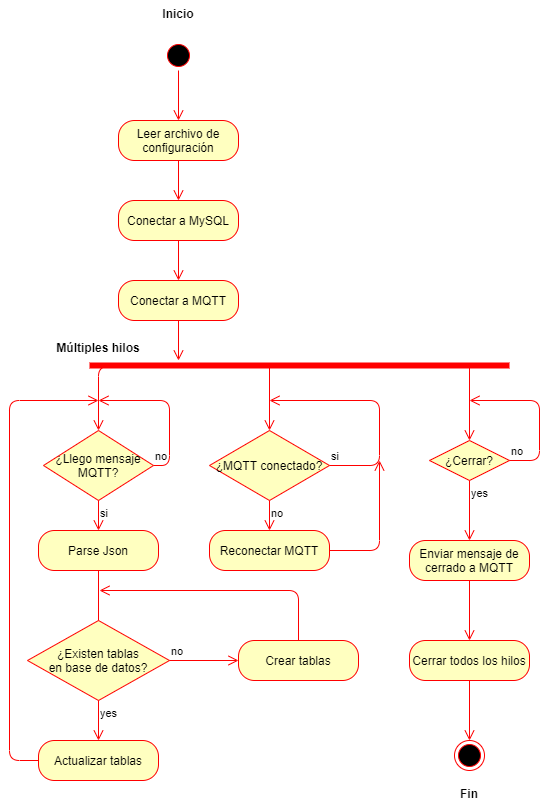
\includegraphics[width=0.8\linewidth]{../imagenes/MQTT-Json --_ MySQL .png} 
				\caption{Diagrama de la aplicación que procesa mensajes.}
				\label{fig:MQTT}
			\end{figure}
			
		
		\subsubsection{Ajuste de Setpoints}
			
			El ajuste de los Setpoints se utilizará para cuando el invernadero funcione tanto con el modelo, como control cerrado o de forma manual. Se realizará mediante una aplicación gráfica desarrollada en Java la cual se muestra en la Figura \ref{fig:proset}. En esta uno seleccionará la variable que desea modificar y su respectivo valor, al enviarse el mensaje se procesará como un mensaje en JSON como los descrito en \ref{parser} y luego enviado por MQTT. Este comportamiento es descrito en mayor detalle en el diagrama de la Figura \ref{fig:diaset}.
			
			
			\begin{figure}[!ht]
				\begin{subfigure}{.5\textwidth}
					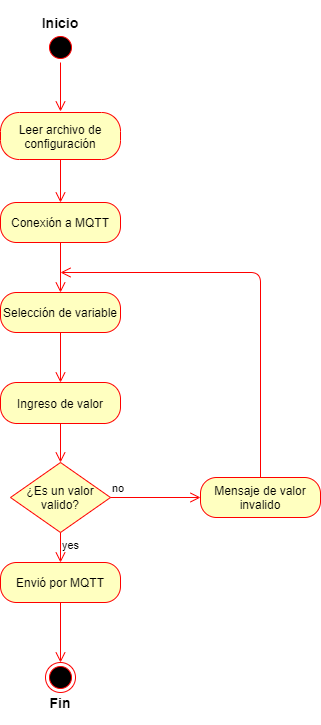
\includegraphics[width=1.\linewidth]{../imagenes/Setpoints .png} 
					\caption{Diagrama del funcionamiento}
					\label{fig:diaset}
				\end{subfigure}
				\begin{subfigure}{.5\textwidth}
					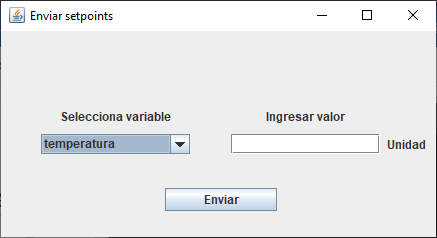
\includegraphics[width=1.\linewidth]{../imagenes/setpoints_programa.PNG}
					\caption{Programa realizado} 
					\label{fig:proset}
				\end{subfigure}
			
			\end{figure}					
		
			
			
			
			
		
%		\subsubsection{Visualizar estados}
		
%			Para la visualización de los estados en el tiempo del invernadero se realiza una interfaz grafica donde se muestra en un grafico la variable seleccionada.
			
			\tarea{Terminar esta aplicación y subir una foto}
	
		\subsubsection{Control lazo cerrado}
			Todos los sistemas anteriores están pensados para funcionar en conjunto, pero en el caso de que alguno de estos falle y que su funcionamiento sea crítico, como lo es el Broker MQTT, se realizó un sistema auxiliar que sirva de respaldo mientras el resto de los sistemas que estén sin funcionamiento. Este sistema está diseñado para realizar un control por lazo cerrado en cada sistema descrito en la \tarea{Figura \ref{Funcionamiento}}, tomando como Setpoint el último entregado por el servidor en el caso de no existir uno que venga por defecto en la programación del ESP32. Cabe destacar, que este control se encontrará dentro de la programación del microcontrolador del invernadero.


	\subsection{Modelo de optimización}
	
		
			\subsubsection{ Descripción del problema}
			
				Se cuenta con un invernadero, el cual tiene de distintos costos relacionados con su funcionamiento. Uno de estos viene dado por la electricidad consumida calefactor en conjunto a la bomba de calefacción $BT*(ebt+ect)$, más el funcionamiento de la bomba de irrigación $BA$, cada uno de estos por sus respectivos costos de electricidad $ce$, otro es el costo del agua $ca$ por el volumen utilizado $BA \cdot aba$ para la irrigación.
	
	Por otro lado, es necesario mantener dentro de un rango la temperatura de agua $\left [ ta_{min},ta_{max} \right ]$, la temperatura del suelo $\left [ tp_{min},tp_{max} \right ]$, la temperatura del aire dentro del invernadero $\left [ tai_{min},tai_{max} \right ]$, y la humedad relativa del suelo entre $\left [ hs_{min},hs_{max} \right ]$.
				

			\subsubsection{Supuestos}
				\begin{enumerate}[label=\roman*.]
					\item	La temperatura del aire dentro y fuera del invernadero es homogénea.
					\item	La temperatura del aire fuera del invernadero puede ser obtenida para una ventana de tiempo determinada.
					\item	La temperatura del agua dentro del contenedor del invernadero es homogénea debido al efecto de la bomba de calefacción.
					\item	La temperatura dentro del tubo de calefacción es homogénea.
					\item	El flujo del calor en la tierra es de forma homogénea respecto a las diferencias de temperatura en los extremos, se asume un suelo ideal con resistencia térmica ideal.
					\item	La tubería de calefacción atraviesa de tal forma cada sub-modulo que se puede asumir un mismo patrón del flujo de calor y por consiguiente emiten la misma cantidad de calor al aire externo.
					\item	Las pérdidas de calor en la plantación por el suelo al exterior son despreciables ya que se encuentran aislado térmicamente.
					\item	Todas las resistencias térmicas en el invernadero no varían respecto a la temperatura, debido a las diferencias máximas de temperatura a las cuales estarán expuestos.
					\item	La recarga de la columna de agua es de forma total, independiente del nivel actual.
					\item	\tarea{investigar esto}Los niveles de humedad relativa que se mantienen en el invernadero permiten despreciar la evo-transpiración.
					\item	La humedad relativa del suelo puede ser determinada por regresión.
					
				\end{enumerate}
				
				
				

			\begin{table}[!ht]
				\centering
				\resizebox{\linewidth}{!}{%
				\begin{tabular}{|ll|}
					\hline
Conjuntos  &                                                                                              \\ \hline
$TIME       $& \{0,maxt\} Conjunto de tiempos distanciados por "periodo" segundos                                                                                      \\
$TIEMPOS    $& \{periodo,maxt\} Sub-conjunto de $TIME$ \\
$VARS       $& \{0,maxt\} Conjunto de variables de holgura para requerimientos de la planta                            \\ \hline
Parametros   &                                                                                              \\ \hline
$periodo    $& Tiempo en segundos que dura cada tiempo                                                      \\
$maxt       $& Numero máximo de tiempos                                                                     \\
$caleagua   $& Calor especifico del agua                                                                    \\
$caleaire   $& Calor especifico del aire                                                                    \\
$masaaire   $& Masa del aire que esta atrapado dentro del invernadero                                       \\
$denagua    $& Densidad del agua                                                                            \\
$rags       $& Resistencia térmica desde el agua a la superficie de la tierra                               \\
$rsai       $& Resistencia térmica desde la superficie de la tierra al aire atrapado                        \\
$raie       $& Resistencia térmica desde el aire atrapado al aire en el exterior                            \\
$tiag       $& Temperatura inicial de agua                                                                  \\
$tiai       $& Temperatura inicial de aire atrapado                                                         \\
$vi         $& Volumen inicial del agua litros                                                              \\
$ceav       $& Calor especifico volumétrico del agua                                                        \\
$qc         $& Calor generado en KJ por encender el calefactor en un tiempo                   \\
$ce         $& Costo en pesos (CLP) por KWh de electricidad consumida                                       \\
$ca         $& Costo en pesos (CLP) por litro de agua consumida                                             \\
$eba        $& Energía consumida en KWh por activar la bomba de irrigación                    \\
$ebt        $& Energía consumida en KWh por activar la bomba de calefacción                   \\
$ect        $& Energía consumida en KWh por activar el calefactor                             \\
$taimin     $& Límite inferior a la temperatura del aire atrapado en C°                                     \\
$taimax     $& Límite superior a la temperatura del aire atrapado en C°                                     \\
$tamax      $& Temperatura máxima a la que calienta el agua el calefactor en C°                             \\
$tamin      $& Temperatura mínima del agua en el sub-modulo central en C°                                   \\
$aba        $& Cantidad de agua en litros que se ocupa al utilizar la bomba de agua                         \\
$Hrel       $& Porcentaje de humedad relativa añadida por una activación de la irrigación                   \\
$Hmin       $& Porcentaje mínimo de humedad en el suelo para la planta                                      \\
$Hmax       $& Porcentaje máximo de humedad para la planta                                                  \\
$Hin        $& Humedad relativa inicial                                                                     \\
$mucho_v$    & Ponderador de holguras CLP/(sobre limite)$v \in VARS$       (costo feo)                      \\
$te_t$       & Temperatura exterior en el tiempo $t \in TIME$                                               \\ \hline
Variables decisión&                                                                                              \\ \hline
$BT_t$       & 1 si se enciende la bomba de temperatura y el calefactor en el tiempo $t \in TIME$ , 0 si no \\
$BA_t$       & 1 si se enciende la bomba de agua en el tiempo $t \in TIME$ , 0 si no                        \\
$VA_t$		 & Volumen de agua en litros en el tiempo $t \in TIME$											\\
$CF_{tv}$	 & Variable de holgura $v \in VARS$ en el tiempo $t \in TIME$ 	(costo feo)						\\ \hline
Variables auxiliares &																						\\ \hline
$HUM_t$      & Porcentaje de humedad relativa en la tierra del invernadero en el tiempo $t \in TIME$        \\ 
$TAI_t$      & Temperatura en C°  del aire atrapado en el tiempo $t \in TIME$                               \\
$TAG_t$      & Temperatura en C°  del agua en el tiempo $t \in TIME$                                        \\ \hline

				\end{tabular}%
				}
				\caption{Conjuntos, parámetros y variables del modelo}
				\label{t:par&var}
			\end{table}		
			
					
				
				
	
				
			\subsubsection{Modelo Matemático}
			
				A continuación, se presenta el modelo matemático:
				
				
				
					\begin{align}
						Min &	\sum_{t \in TIEMPOS}^{}( ce*( BT_t*(ebt + ect)))&+\label{f:electricidad}\\
							&	\sum_{t \in TIEMPOS}^{}( ca*BA_t*aba )&+\label{f:agua}\\
							&	\sum_{v \in VARS}^{}\sum_{t \in TIEMPOS}^{}(mucho_v*CF_{t,v} )&\label{f:holgura}
					\end{align}
					
				


La función \ref{f:electricidad} minimiza el consumo eléctrico debido a las activaciones de bombas y el calefactor y la función \ref{f:agua} minimiza el gasto en agua, en ambos casos se relacionan el consumo a una unidad monetaria además se agrega un holgura figura \ref{f:holgura} por situaciones en que el sistema no es capaz de mantener las condiciones mínimas y/o máximas.


				
				
				
				
				
				
				
				
				
				
			
			
					\begin{align}
						 TAG_t	=	TAG_{t-p}+	&((BT_{t-p}*qc*1000 + 
						\nonumber						  \\&8*  \frac{TAI_{t-p}-TAG_{t-p}}{rags+rsai}   )
						\nonumber						  \\&* \frac{p}{VA_t*caleagua*denagua}) 		&\forall \;  p=periodo \; , \; t \in TIME			\label{f:temp_agua}\\
						\nonumber\\
						TAI_t	= 	TAI_{t-p}- &(\frac{8*(TAI_{t-p}-TAG_{t-p}}{rags+rsai}+ 
                        \nonumber                       \\&\frac{te_{t-p}-TAI_{t-p}}{raie} ) *
						\nonumber						 \\&\frac{p}{masaaire*caleaire}			&\forall \; p=periodo \; , \; t \in TIME		\label{f:temp_aire}
					\end{align}		
					
					
											
			
				La restricción \ref{f:temp_agua} representa la transferencia de calor desde el calefactor al agua dentro del estanque, además de la transferencia hacia el aire interno a través de los 8 contenedores con tierra, de igual manera, la restricción \ref{f:temp_aire} representa las transferencias desde el aire interno y hacia el exterior del invernadero.

				\duda{agrego lo que esta comentado para explicar las transferencias o lo paso a marco teórico}
				
%				Cada temperatura en el tiempo se calculará según la ecuación \ref{eq:delta_t}.
%	Donde $\Delta \dot{Q}$ representa la transferencia de calor neta, $p$ representa el periodo entre cada tiempo (en segundos), $Cm$ representa el calor específico del material y $m$ representa la masa del material involucrado en la transferencia de calor. Además, cada flujo de calor, a excepción del generado por el calefactor, puede ser calculando según la ecuación \ref{eq:delta_q} donde la $R$ corresponde a la resistencia térmica y $T$ es la temperatura.
%				
%				
%				
%				\begin{equation}
%				 \dot{Q} = \frac{T_{1}-T_{2}}{R}
%				\label{eq:delta_q}
%				\end{equation}
				
				
				
				
				
				\begin{align}
					HUM_t	&<= 	HUM_{t-p} + Fe+BA_t*Hrel											&\forall \; p=periodo \; , \; t \in TIME			\label{f:consumo_agua}	\\
					VA_t	&=	VA_{t-p} - aba*BA_{t-p}										&\forall \; p=periodo \; , \; t \in TIME			\label{f:rel_bomba_irigar}
				\end{align}
					
				La restricción \ref{f:consumo_agua} modela las variaciones de la humedad relativa en el suelo en función de las activaciones de $BA_t$ y de la disminución de humedad característica del sistema $Fe$. Además  la restricción \ref{f:rel_bomba_irigar} relaciona el consumo de agua con las activaciones de la bomba de irrigación.
				
				
				
				
				

				\begin{align}
					var_t	  &<=	var_max	+CF_{t,v}		&\forall \;t \in \; TIME\label{f:var_min}\\
					var_min   &<=  var_t	+CF_{t,v}		&\forall \;t \in \; TIME\label{f:var_max}
				\end{align}





				Las restricciones \ref{f:var_min} y \ref{f:var_max} representan de forma genérica la utilización de holguras $CF_{t,v}$ sobre cada variable auxiliar $var_t$ (\ref{t:par&var}) en cada tiempo $t$ para evitar que las temperatura y humedades salgan de los rangos impuestos según la planta a cultivar.
				
				
				
				\begin{align}
					TAI_t \,=&\; tiai			&\forall \; t = 0\nonumber\\
					TAG_t \,=&\; tiag			&\forall \; t = 0\label{f:c_iniciales}\\
					HUM_t \,=&\; Hin				&\forall \; t = 0\nonumber
				\end{align}
				
				
				El grupo de restricciones \ref{f:c_iniciales} entregan las condiciones iniciales al modelo.
				
				
				
				
				
				
				 
				\begin{align}
					&BT_t \, , \, BA_t \, , \, VA_t \, , \, CF_{tv} \, \in \{1,0\}				&\forall \; t \in TIEMPOS \label{DOM_decicion} \\
					&TAI_t \, , \, TAG_t \, \in {\rm I\!R}										&\forall \; t \in TIME \label{DOM_aux1} \\
					&HUM_t \, \in \{100,0\}														&\forall \; t \in TIME \label{DOM_aux2}
				\end{align}

	
				Las restricciones \ref{DOM_decicion}, \ref{DOM_aux1}, \ref{DOM_aux2} indican el dominio de las variables.